\documentclass[10pt]{beamer}
\usepackage{amsmath}
\usepackage{mathtools}
\usefonttheme{professionalfonts} % using non standard fonts for beamer
\usefonttheme{serif} % default family is serif

%\documentclass[12pt]{beamerthemeSam.sty}
\usepackage{epsf}
%\usepackage{pstricks}
%\usepackage[orientation=portrait,size=A4]{beamerposter}
\geometry{paperwidth=160mm,paperheight=120mm}
%DT favorite definitions
\def\LL{\left\langle}	% left angle bracket
\def\RR{\right\rangle}	% right angle bracket
\def\LP{\left(}		% left parenthesis
\def\RP{\right)}	% right parenthesis
\def\LB{\left\{}	% left curly bracket
\def\RB{\right\}}	% right curly bracket
\def\PAR#1#2{ {{\partial #1}\over{\partial #2}} }
\def\PARTWO#1#2{ {{\partial^2 #1}\over{\partial #2}^2} }
\def\PARTWOMIX#1#2#3{ {{\partial^2 #1}\over{\partial #2 \partial #3}} }

\def\rightpartial{{\overrightarrow\partial}}
\def\leftpartial{{\overleftarrow\partial}}
\def\diffpartial{\buildrel\leftrightarrow\over\partial}

\def\BI{\begin{itemize}}
\def\EI{\end{itemize}}
\def\BE{\begin{displaymath}}
\def\EE{\end{displaymath}}
\def\BEA{\begin{eqnarray*}}
\def\EEA{\end{eqnarray*}}
\def\BNEA{\begin{eqnarray}}
\def\ENEA{\end{eqnarray}}
\def\EL{\nonumber\\}
\def\BCC{\begin{columns}}
\def\ECC{\end{columns}}
\def\HC{\column{0.5\textwidth}}

\newcommand{\map}[1]{\frame{\frametitle{\textbf{Course map}}
\centerline{\includegraphics[height=0.86\paperheight]{../../map/#1.png}}}}
\newcommand{\wmap}[1]{\frame{\frametitle{\textbf{Course map}}
\centerline{\includegraphics[width=0.96\paperwidth]{../../map/#1.png}}}}

\newcommand{\etal}{{\it et al.}}
\newcommand{\gbeta}{6/g^2}
\newcommand{\la}[1]{\label{#1}}
\newcommand{\ie}{{\em i.e.\ }}
\newcommand{\eg}{{\em e.\,g.\ }}
\newcommand{\cf}{cf.\ }
\newcommand{\etc}{etc.\ }
\newcommand{\atantwo}{{\rm atan2}}
\newcommand{\Tr}{{\rm Tr}}
\newcommand{\dt}{\Delta t}
\newcommand{\op}{{\cal O}}
\newcommand{\msbar}{{\overline{\rm MS}}}
\def\chpt{\raise0.4ex\hbox{$\chi$}PT}
\def\schpt{S\raise0.4ex\hbox{$\chi$}PT}
\def\MeV{{\rm Me\!V}}
\def\GeV{{\rm Ge\!V}}

%AB: my color definitions
%\definecolor{mygarnet}{rgb}{0.445,0.184,0.215}
%\definecolor{mygold}{rgb}{0.848,0.848,0.098}
%\definecolor{myg2g}{rgb}{0.647,0.316,0.157}
\definecolor{abtitlecolor}{rgb}{0.0,0.255,0.494}
\definecolor{absecondarycolor}{rgb}{0.0,0.416,0.804}
\definecolor{abprimarycolor}{rgb}{1.0,0.686,0.0}
\definecolor{Red}           {cmyk}{0,1,1,0}
\definecolor{Grey}           {cmyk}{.7,.7,.7,0}
\definecolor{Blue}          {cmyk}{1,1,0,0}
\definecolor{Green}         {cmyk}{1,0,1,0}
\definecolor{Brown}         {cmyk}{0,0.81,1,0.60}
\definecolor{Black}         {cmyk}{0,0,0,1}

\usetheme{Madrid}


%AB: redefinition of beamer colors
%\setbeamercolor{palette tertiary}{fg=white,bg=mygarnet}
%\setbeamercolor{palette secondary}{fg=white,bg=myg2g}
%\setbeamercolor{palette primary}{fg=black,bg=mygold}
\setbeamercolor{title}{fg=abtitlecolor}
\setbeamercolor{frametitle}{fg=abtitlecolor}
\setbeamercolor{palette tertiary}{fg=white,bg=abtitlecolor}
\setbeamercolor{palette secondary}{fg=white,bg=absecondarycolor}
\setbeamercolor{palette primary}{fg=black,bg=abprimarycolor}
\setbeamercolor{structure}{fg=abtitlecolor}

\setbeamerfont{section in toc}{series=\bfseries}

%AB: remove navigation icons
\beamertemplatenavigationsymbolsempty
\title[A few notes on bars and drums]{
  \textbf {A few notes on bars and drums}\\
%\centerline{}
%\centering
%\vspace{-0.0in}
%\includegraphics[width=0.3\textwidth]{propvalues_0093.pdf}
%\vspace{-0.3in}\\
%\label{intrograph}
}

\author[W. Freeman] {Physics 200\\Syracuse University, Physics 200 Spring 2018\\Walter Freeman}

\date{\today}

\begin{document}

\frame{\titlepage}

\frame{
\BCC

\HC\begin{center} 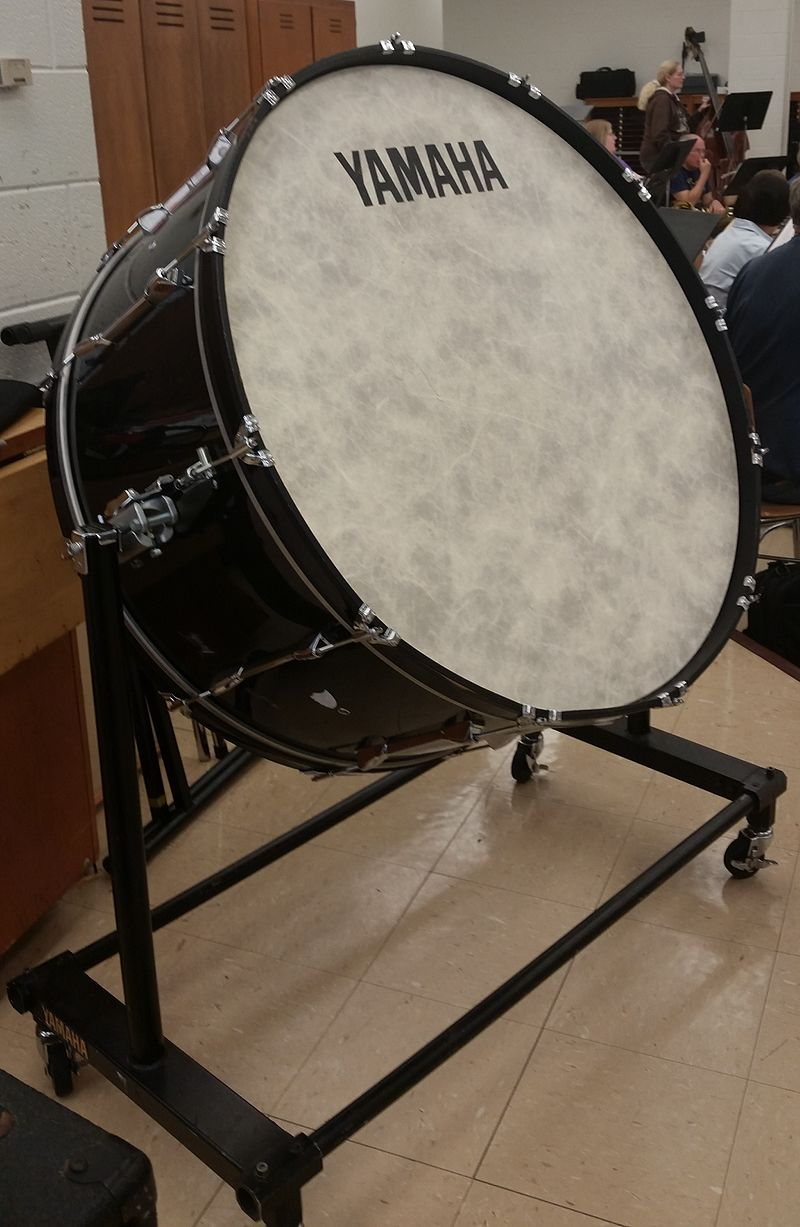
\includegraphics[width=0.4\textwidth]{bass-drum-1.jpg}\end{center}
\HC\begin{center} 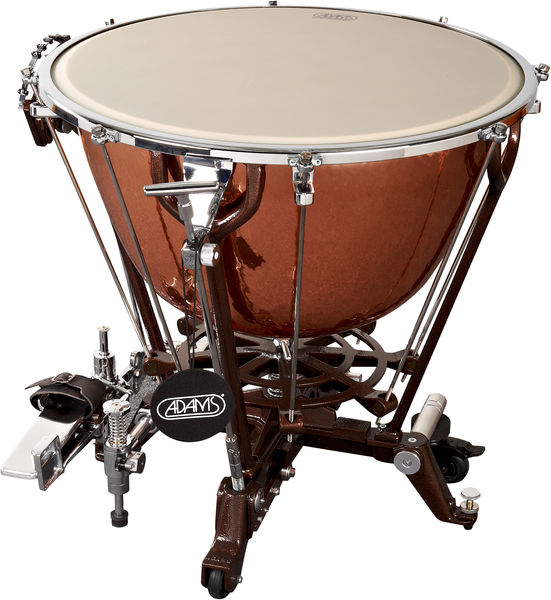
\includegraphics[width=0.6\textwidth]{timpani.jpg}\end{center}
\ECC

\begin{center}
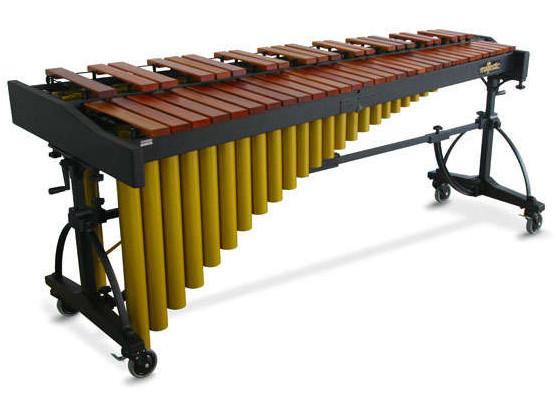
\includegraphics[width=0.4\textwidth]{marimba.jpg}
\end{center}
}

\frame{
\Large
\begin{center}
How do we make musical notes with a metal/wooden bar?

\bigskip
\bigskip

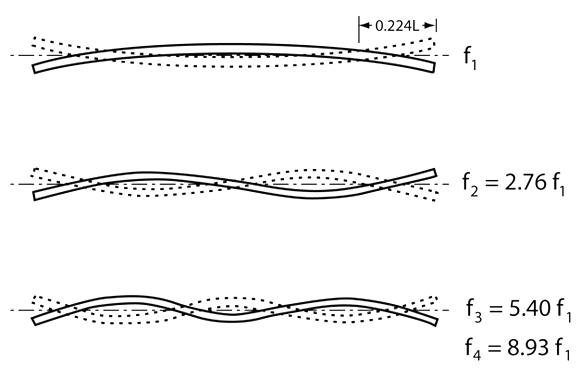
\includegraphics[width=0.6\textwidth]{bar-modes.png}

\bigskip
\bigskip

\pause

I'll let you all figure this one out!
\end{center}
}

\frame{
\Large
\begin{center}
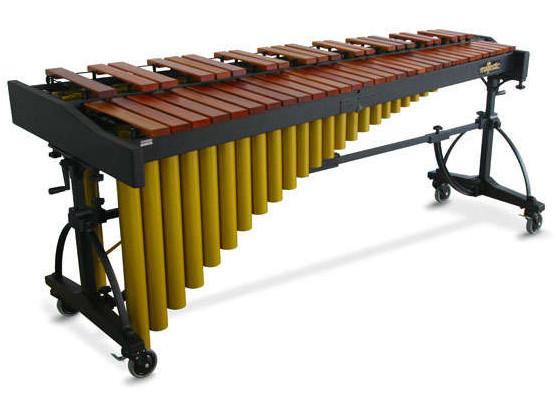
\includegraphics[width=0.5\textwidth]{marimba.jpg}
\bigskip
\bigskip
\end{center}
\begin{itemize}
  \item Glockenspiel (``bell-player''): bars made of metal

  \item Xylophone (``wood-sound''): bars made of wood

  \item Marimba: additional resonating tubes near each bar to amplify fundamental

  \item Vibraphone: use a motor to move things around in the tubes, creating vibrato/tremolo
\end{itemize}
}

\frame{
\Large
\begin{center}
How does a circular membrane vibrate?

  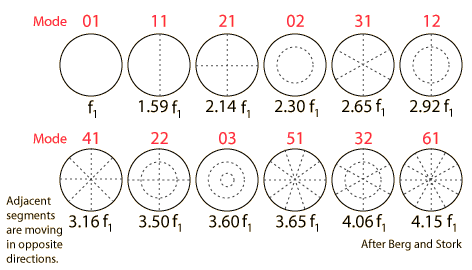
\includegraphics[width=0.8\textwidth]{membrane-modes.png}

\pause
\pause

This is not a harmonic series...

\end{center}
}

  \frame{
    \Large
How do we make harmony out of this mess?

\BI
\item Some modes might be suppressed (as in the marimba)
  \BI
\item Turns out radially-symmetric ones are suppressed strongly, particularly (0,1)
\item Other modes can be suppressed by beating at a nodal point
  \EI
\item  ``Retune'' the others by modifying the membrane?
  \EI
}

  \frame{
\BCC
\HC
\large
Largest effect: coupling between membrane and vibration of air

\bigskip

  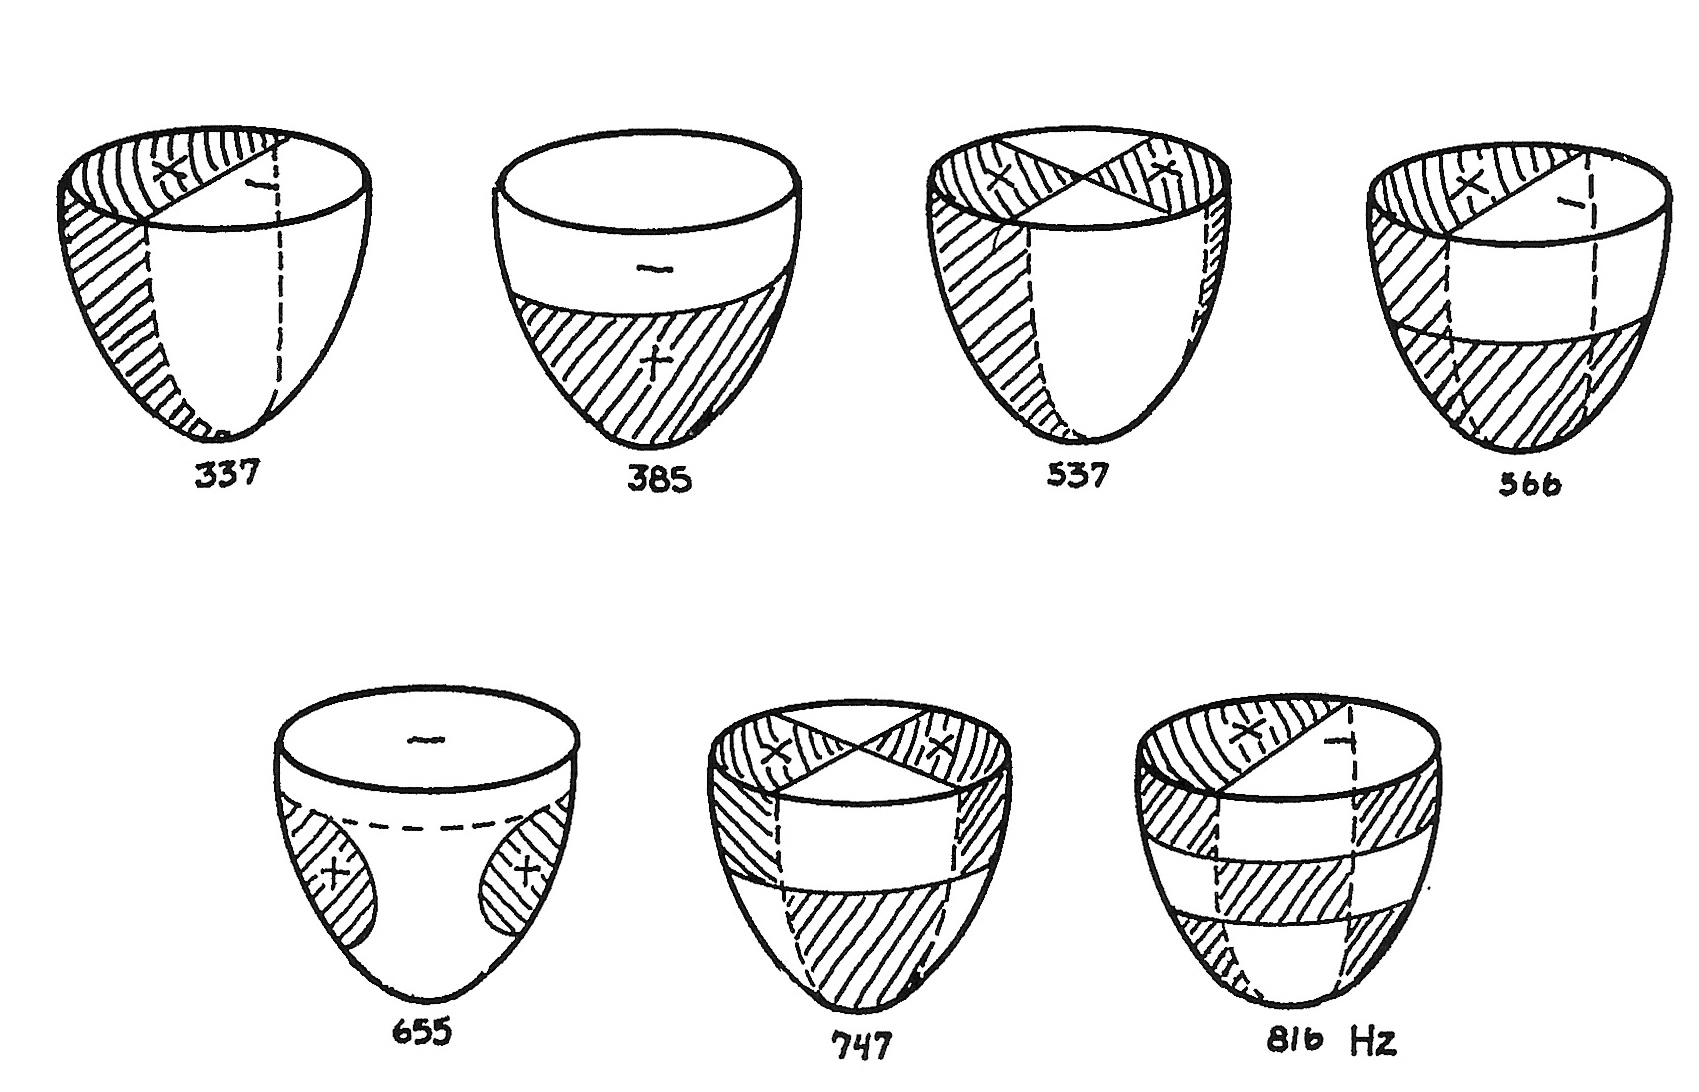
\includegraphics[width=\textwidth]{Air-Modes-Kettle.jpg}

\bigskip

  Another effect: not-quite-uniform tension across the head

\HC
\begin{tabular}{c|c|c}
  Mode & Theoretical & Actual \\
  0,1 & --- & --- \\
  \bf 1,1 &\bf  1.00 &\bf  1.00 \\
  \bf 2,1 &\bf  1.35 & \bf 1.504 \\
  0,2 & --- & 1.742 \\
  \bf 3,1 &\bf  1.67 & \bf 2.000 \\
  1,2 & --- & 2.245 \\
  \bf 4,1 & \bf 1.99 &\bf  2.494 \\
  2,2 & --- & 2.800 \\
  0,3 & --- & 2.852 \\
  \bf 5,1 & \bf 2.30 & \bf 2.979 \\
  \bf 6,1 & \bf 2.61 & \bf 3.462 \\
\end{tabular}
\ECC
}

\end{document}
